\subsection{Houses}
\label{subsec:application:building_the_model:houses}

The first step of building the model is to add a type. Without any types, nothing interesting can be produced. The first type will be the class type for houses. \cref{subsec:library_of_transformations:type_level_transformations:regular_classes} is used to introduce the class type, while on the instance level, \cref{subsec:library_of_transformations:instance_level_transformations:plain_objects} is used to introduce the house objects.

The $name$ of the new house type is $.\type{House}$. Furthermore, 2 house objects are introduced, $objects = \{TR, BHP\}$. Furthermore, we assume that the object identifiers are equal to the internal node id, so $fid(TR) = TR$ and $fid(BHP) = BHP$. The following model is obtained:

\LTXtable{\textwidth}{tex/06_application/02_building_the_model/tables/01_houses.tex}

\begin{figure}[p]
    \centering
    \begin{subfigure}{0.98\textwidth}
        \centering
        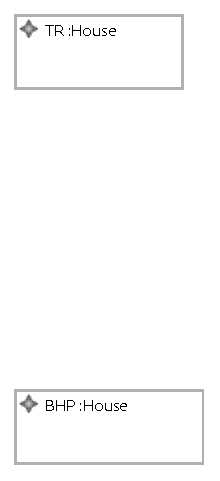
\includegraphics{images/06_application/instance_model/step01.pdf}
        \caption{Instance Model $Im_1$}
        \label{fig:application:building_the_model:houses:ecore:instance_model}
    \end{subfigure}
    \\
    \begin{subfigure}{0.98\textwidth}
        \centering
        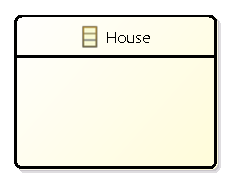
\includegraphics{images/06_application/type_model/step01.pdf}
        \caption{Type Model $Tm_1$}
        \label{fig:application:building_the_model:houses:ecore:type_model}
    \end{subfigure}
    \caption{The Ecore model after step 1}
    \label{fig:application:building_the_model:houses:ecore}
\end{figure}

\begin{figure}[p]
    \centering
    \begin{subfigure}{0.98\textwidth}
        \centering
        % To use this figure in your LaTeX document
% import the package groove/resources/groove2tikz.sty
%
\begin{tikzpicture}[scale=\tikzscale,name prefix=step01-]
\node[type_node] (n0) at (0.530, -0.370) {\ml{\textbf{House}}};

\end{tikzpicture}

        \caption{Instance Graph $IG_1$}
        \label{fig:application:building_the_model:houses:groove:instance_graph}
    \end{subfigure}
    \\
    \begin{subfigure}{0.98\textwidth}
        \centering
        % To use this figure in your LaTeX document
% import the package groove/resources/groove2tikz.sty
%
\begin{tikzpicture}[scale=\tikzscale,name prefix=step01-]
\node[type_node] (n0) at (0.530, -0.370) {\ml{\textbf{House}}};

\end{tikzpicture}

        \caption{Type Graph $TG_1$}
        \label{fig:application:building_the_model:houses:groove:type_graph}
    \end{subfigure}
    \caption{The GROOVE graphs after step 1}
    \label{fig:application:building_the_model:houses:groove}
\end{figure}

A visual representation of $Tm_1$ and $Im_1$ can be found in \cref{fig:application:building_the_model:houses:ecore}. Similarly, a visual representation of $TG_1$ and $IG_1$ can be found in \cref{fig:application:building_the_model:houses:groove}. Please note that because of the definitions of $f_1(Im_1)$ and $f'_1(IG_1)$, we have that $f_1(Im_1) = IG_1$ and $f'_1(IG_1) = Im_1$. Furthermore, $f_1(Im_1)$ and $f'_1(IG_1)$ are valid mapping functions themselves, such that they can be combined with another mapping function in the next step.

The models itself are not very special as of yet, but that is expected. Each step is only a small building block, and introducing a type is not very special.

\afterpage{\FloatBarrier}